\subsection{数学期望}
\subsubsection{例子}
\paragraph{}
\textbf{例子\;}一射手进行打靶练习,规定射入区域$e_2$得2分,射入区域$e_1$得1分,脱靶,即射入区域$e_0$,得0分。射手一次射击得分数$X$是一个随机变量。设$X$的分布律为

\begin{equation*}
  P\{X=k\}=p_k, \; k = 0,1,2.
\end{equation*}

\begin{figure}[H]
\centering
  % 打靶练习
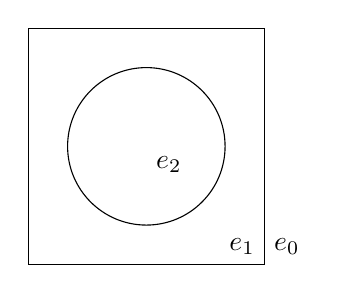
\begin{tikzpicture}
  \draw (-1.5,-1.5) rectangle (1.5,1.5);
  \draw (0,0) circle [radius=1];

  \node[below right] at (0,0) {$e_2$};
  \node[above left] at (1.5,-1.5) {$e_1$};
  \node[above right] at (1.5,-1.5) {$e_0$};
\end{tikzpicture}

  \caption{打靶练习}
  \label{打靶练习}
\end{figure}

\paragraph{}
现在射击$N$次,其中得0分的有$a_0$次,得1分的有$a_1$次,得2分的有$a_2$次,$a_0+a_1+a_2=N$。他射击$N$次得分的总和为$a_0 \times 0 + a_1 \times 1 + a_2 \times 2$。于是平均一次射击的得分数为
\begin{equation*}
  \frac{a_0 \times 0 + a_1 \times 1 + a_2 \times 2}{N} = \sum_{k=0}^2 k \frac{a_k}{N}.
\end{equation*}

\paragraph{}
这里,$\displaystyle \frac{a_k}{N}$是事件$\{X=k\}$的频率。当$N$很大时,$\displaystyle \frac{a_k}{N}$在一定意义下接近于事件$\{X=k\}$的概率$p_k$。就是说,在试验次数很大时,随机变量$X$的观察值的算术平均$\displaystyle \sum_{k=0}^2 k \frac{a_k}{N}$在一定意义下接近于$\displaystyle \sum_{k=0}^2 kp_k$。我们称$\displaystyle \sum_{k=0}^2 kp_k$为随机变量$X$的数学期望或均值。

\subsubsection{定义}
\paragraph{}
\textbf{定义\;}设离散型随机变量$X$的分布律为

\begin{equation*}
  P\{X=x_k\} = p_k, \; k = 1,2,\cdots.
\end{equation*}

若级数
\begin{equation*}
  \sum_{k=1}^\infty x_k p_k
\end{equation*}

绝对收敛,则称级数$\displaystyle \sum_{k=1}^\infty x_k p_k$的和为随机变量$X$的\textbf{数学期望},记为$E(X)$。即

\begin{equation}
  \label{离散型随机变量的数学期望}
  E(X) = \sum_{k=1}^\infty x_k p_k
\end{equation}

\paragraph{}
设连续型随机变量$X$的概率密度为$f(x)$,若积分

\begin{equation*}
  \int_{-\infty}^\infty xf(x)dx
\end{equation*}

绝对收敛,则称积分$\displaystyle \int_{-\infty}^\infty xf(x)dx$的值为随机变量$X$的\textbf{数学期望},记为$E(X)$。即

\begin{equation}
  \label{随机型随机变量的数学期望}
  E(X)=\int_{-\infty}^\infty xf(x)dx
\end{equation}

\paragraph{}
数学期望简称\textbf{期望},又称为\textbf{均值}。

\subsubsection{定理}
\paragraph{}
\textbf{定理\;}设$Y$是随机变量$X$的函数:$Y=g(X)$($g$是连续函数)。
\begin{enumerate}
  \item 如果$X$是离散型随机变量,它的分布律为$P\{X=x_k\}=p_k, \; k = 1,2,\cdots,$若$\displaystyle \sum_{k=1}^\infty g(x_k)p_k$绝对收敛,则有
  \begin{equation}
    E(Y)=E[g(X)]=\sum_{k=1}^\infty g(x_k)p_k.
  \end{equation}
  \item 如果$X$是连续型随机变量,它的概率密度为$f(x)$,若$\displaystyle \int_{-\infty}^\infty g(x)f(x)dx$绝对收敛,则有
  \begin{equation}
    E(Y) = E[g(X)] = \int_{-\infty}^\infty g(x)f(x)dx.
  \end{equation}
\end{enumerate}

\paragraph{}
定理的重要意义在于当我们求$E(Y)$时,不必算出$Y$的分布律或概率密度,而只需利用$X$的分布律或概率密度就可以了。

\subsubsection{性质}
\paragraph{}
\begin{enumerate}
  \item 设$C$是常数,则有$E(C)=C$。
  \item 设$X$是一个随机变量,$C$是常数,则有$E(CX)=CE(X)$。
  \item 设$X,Y$是两个随机变量,则有$E(X+Y)=E(X) + E(Y)$。这一性质可以推广到任意有限个随机变量之和的情况。
  \item 设$X,Y$是\textbf{相互独立的}随机变量,则有$E(XY)=E(X)E(Y)$。这一性质可以推广到任意有限个\textbf{相互独立的}随机变量之积的情况。
\end{enumerate}

\subsection{方差}
\subsubsection{例子}
\paragraph{}
例如,有一批灯泡,知其平均寿命是$E(X)=1\,000$(小时)。仅由这一指标我们还不能判断这批灯泡的质量好坏。还需进一步考察灯泡寿命$X$与其均值$E(X)=1\,000$的\textbf{偏离程度}。若偏离程度较小,表示质量比较稳定。容易看到

\begin{equation*}
  E\{|X-E(X)|\}
\end{equation*}

能度量随机变量与其均值$E(X)$的偏离程度。但由于上式带有绝对值,运算不方便,为运算方便起见,通常用量
\begin{equation*}
  E\{[X-E(X)]^2\}
\end{equation*}
来度量随机变量$X$与其均值$E(X)$的偏离程度。

\subsubsection{定义}
\paragraph{}
\textbf{定义\;}设$X$是一个随机变量,若$E\{[X-E(X)]^2\}$存在,则称$E\{[X-E(X)]^2\}$为$X$的\textbf{方差},记为$D(X)$或$Var(X)$,即
\begin{equation}
  D(X)=Var(X)=E\{[X-E(X)]^2\}.
\end{equation}

\paragraph{}
在应用上还引入量$\sqrt{D(X)}$,记为$\sigma(X)$,称为\textbf{标准差}或\textbf{均方差}。

\paragraph{}
$D(X)$是刻画$X$取值分散程度的一个量,它是衡量$X$取值分散程度的一个尺度。

\paragraph{}
由定义知,方差是随机变量$X$的函数$g(X)=(X-E(X))^2$的数学期望。于是对于离散型随机变量,按\eqref{离散型随机变量的数学期望}式有:
\begin{equation}
  D(X) = \sum_{k=1}^\infty[x_k - E(X)]^2p_k,
\end{equation}
其中$P\{X=x_k\}=p_k,\;k=1,2,\cdots$是$X$的分布律。

\paragraph{}
对于连续型随机变量,按\eqref{随机型随机变量的数学期望}式有:
\begin{equation}
  D(X) = \int_{-\infty}^\infty [x - E(X)]^2f(x)dx,
\end{equation}
其中$f(x)$是$X$的概率密度。

\paragraph{}
随机变量$X$的方差可按下列公式计算:
\begin{equation}
  D(X)=E(X^2)-[E(X)]^2.
\end{equation}

\paragraph{}
设随机变量$X$具有数学期望$E(X)=\mu$,方差$D(X)=\sigma^2 \neq 0$。记
\begin{equation}
  X^* = \frac{X-\mu}{\sigma},
\end{equation}
则
\begin{align*}
  E(X^*) =&\, \frac{1}{\sigma}E(X-\mu)=\frac{1}{\sigma}[E(X)-\mu] = 0; \\
  D(X^*) =&\, E(X^{*2}) - [E(X^*)]^2 = E\Big[\Big(\frac{X-\mu}{\sigma}\Big)^2\Big] \\
         =&\, \frac{1}{\sigma^2}E[(X-\mu)^2]=\frac{\sigma^2}{\sigma^2} = 1
\end{align*}
即$\displaystyle X^* = \frac{X-\mu}{\sigma}$ 的数学期望为$0$,方差为$1$。$X^*$称为$X$的\textbf{标准化变量}。

\subsubsection{性质}
\paragraph{}
性质
\begin{enumerate}
  \item 设$C$是常数,则$D(C)=0$.
  \item 设$X$是随机变量,$C$是常数,则有
  \begin{equation*}
    D(CX) = C^2D(X), \; D(X+C)=D(X).
  \end{equation*}
  \item 设$X,Y$是两个随机变量,则有
  \begin{equation*}
    D(X+Y) = D(X) + D(Y) + 2E\{(X-E(X))(Y-E(Y))\}.
  \end{equation*}
  特别,若$X,Y$相互独立,则有
  \begin{equation*}
    D(X+Y) = D(X) + D(Y).
  \end{equation*}
  \item $D(X)=0$的充要条件是$X$以概率$1$取常数$E(X)$,即
  \begin{equation*}
    P\{X=E(X)\} = 1.
  \end{equation*}
\end{enumerate}

\subsubsection{定理}
\paragraph{}
\textbf{定理\;}设随机变量$X$具有数学期望$E(X)=\mu$,方差$D(X)=\sigma^2$,则对于任意正数$\varepsilon$,不等式
\begin{equation}
  P\{|X-\mu| \geq \varepsilon \} \leq \frac{\sigma^2}{\varepsilon^2}
\end{equation}
成立。

\paragraph{}
这一不等式称为\textbf{切比雪夫(Chebyshev)不等式}。

\paragraph{}
\textbf{意义\;}该不等式给出了在随机变量的分布未知,而只知道$E(X)$和$D(X)$的情况下估计概率$P\{|X-E(X)|<\varepsilon\}$的界限。
\paragraph{}
这个估计是比较粗糙的,如果已经知道随机变量的分布时,那么所需求的概率可以确切地计算出来,也就没有必要利用这一不等式来作估计了。

\subsection{协方差及相关系数}
\paragraph{}

\subsection{矩、协方差矩阵}
\paragraph{}
